\subsection{Isosurface extraction\pavol{update plot text to isosurface}}\label{sec:isocontour}

\begin{figure*}[h]
	\centering
	\subcaptionbox{\em pressure, isovalue=0.2}
	{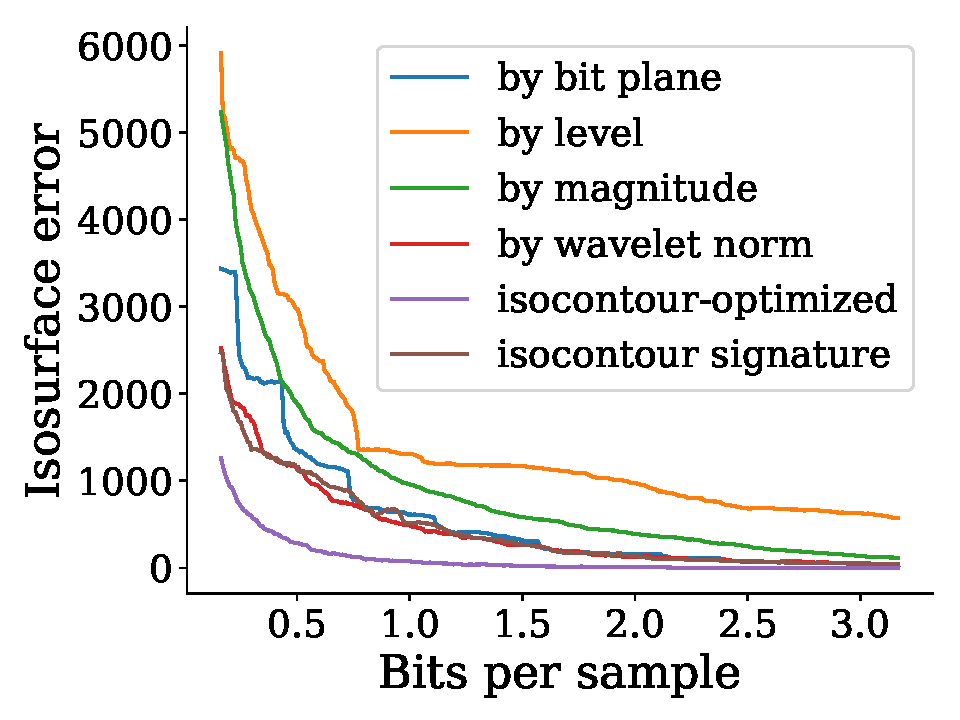
\includegraphics[width=0.24\linewidth]{isocontour/isocontour-optimized-pressure}}
	\subcaptionbox{\em turbulence, isovalue=5}
	{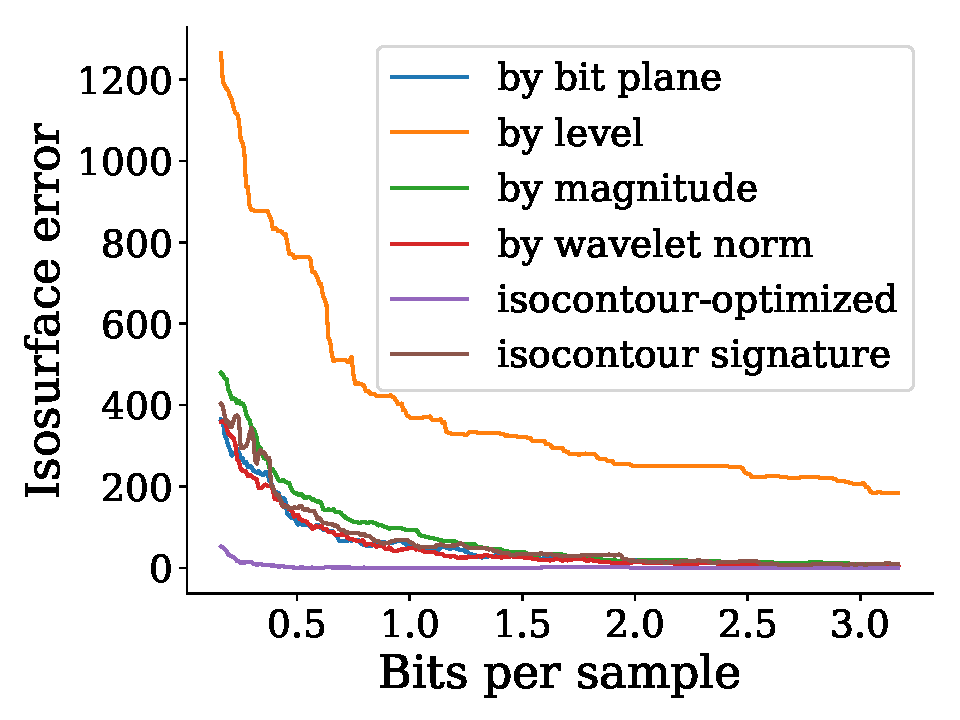
\includegraphics[width=0.24\linewidth]{isocontour/isocontour-optimized-turbulence}}
	\subcaptionbox{\em plasma, isovalue=2}
	{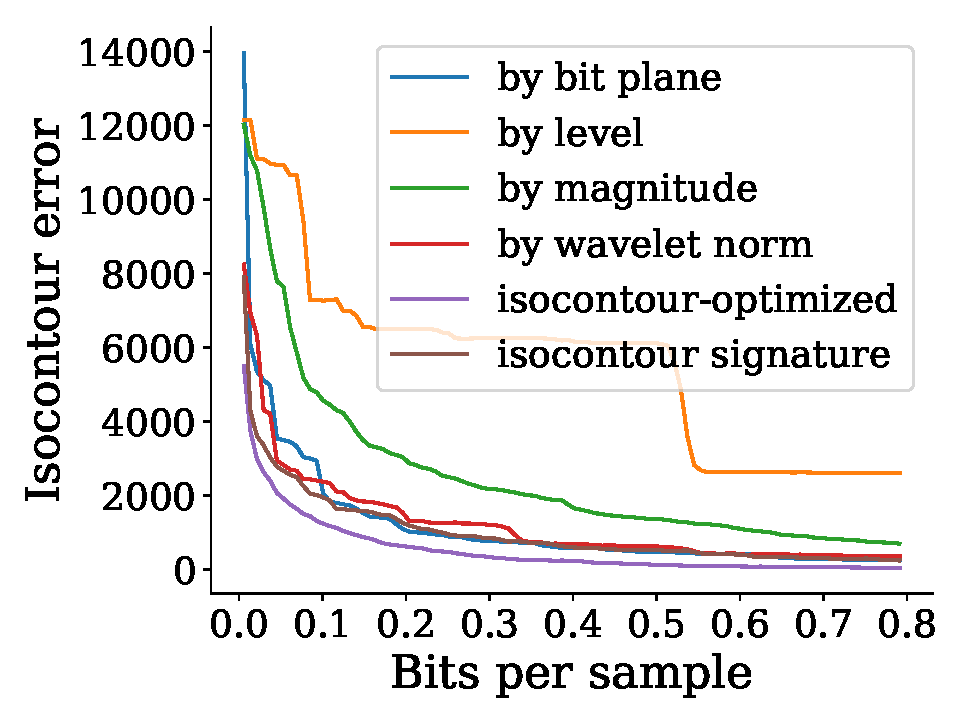
\includegraphics[width=0.24\linewidth]{isocontour/isocontour-optimized-plasma}}
	\subcaptionbox{\em diffusivity, isovalue=-0.05}
	{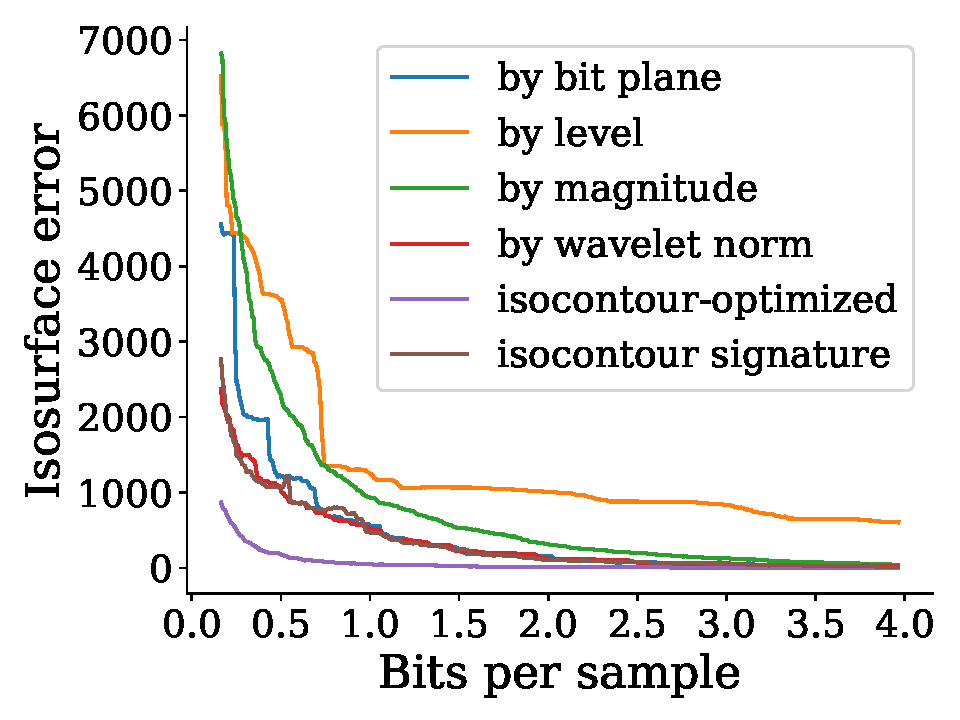
\includegraphics[width=0.24\linewidth]{isocontour/isocontour-optimized-diffusivity}}
	\caption{Comparison of isocontour errors among streams. Plots are truncated to highlight
	differences without hiding important trends. In all cases, $s_{lvl}$ and $s_{mag}$ perform
	significantly worse than the rest. For \emph{pressure} and \emph{diffusivity}, $s_{iso-sig}
	\approx s_{wav} > s_{bit}$. For \emph{plasma}, there are crossovers between $s_{bit}$ and
	$s_{wav}$. Finally, for \emph{turbulence}, $s_{bit} > s_{wav}\approx
	s_{sig}$.}\label{fig:isocontour-plots}
\vspace{1em}

	\centering
	\subcaptionbox{\emph{by level} ($s_{lvl}$)}
	{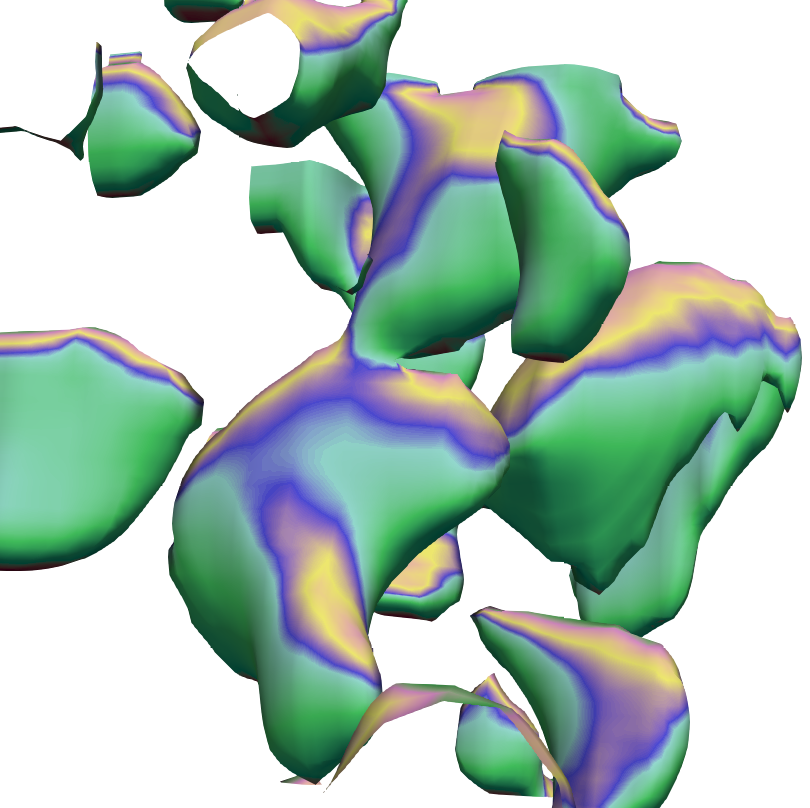
\includegraphics[width=0.16\linewidth]{isocontour/isocontour-level}}
	\subcaptionbox{\emph{by bit plane} ($s_{bit}$)}
	{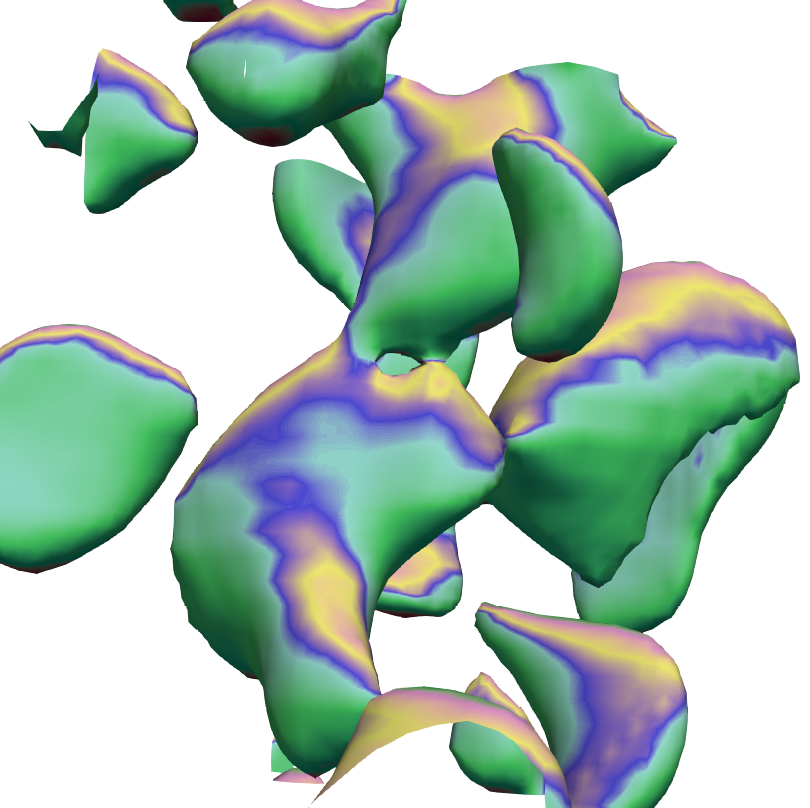
\includegraphics[width=0.16\linewidth]{isocontour/isocontour-bit-plane}}
	\subcaptionbox{\emph{by wavelet norm} ($s_{wav}$)}
	{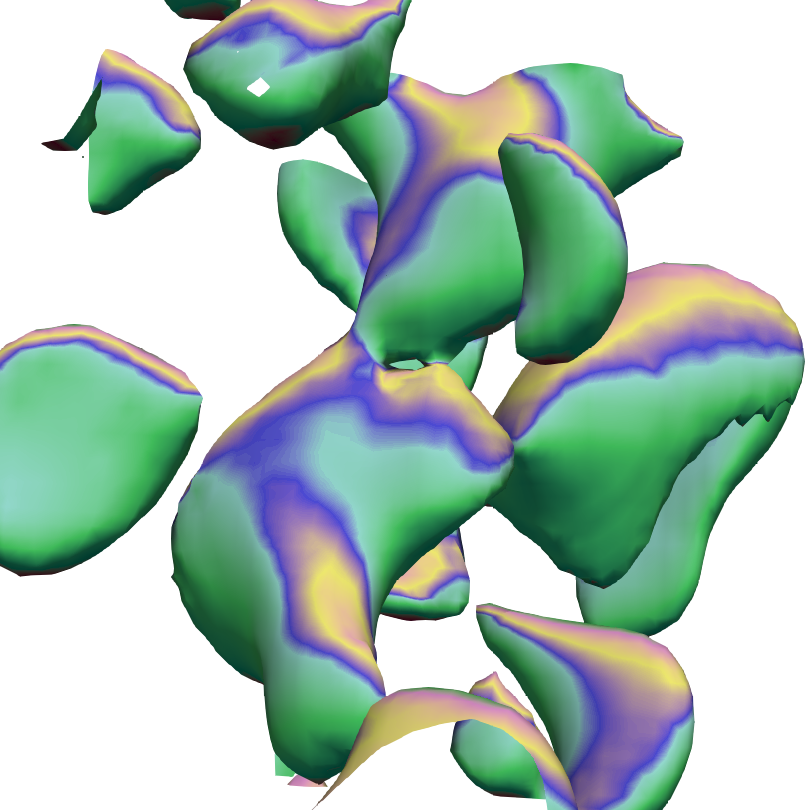
\includegraphics[width=0.16\linewidth]{isocontour/isocontour-wavelet-norm}}
	\subcaptionbox{\emph{by magnitude} ($s_{mag}$)}
	{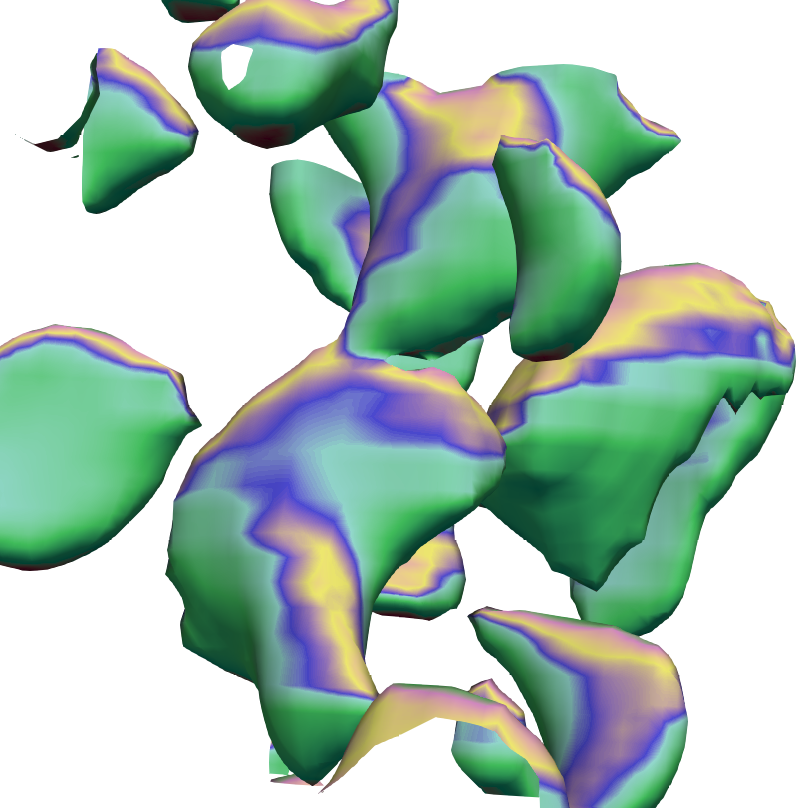
\includegraphics[width=0.16\linewidth]{isocontour/isocontour-magnitude}}
	\subcaptionbox{\emph{by signature} ($s_{iso-sig}$)}
	{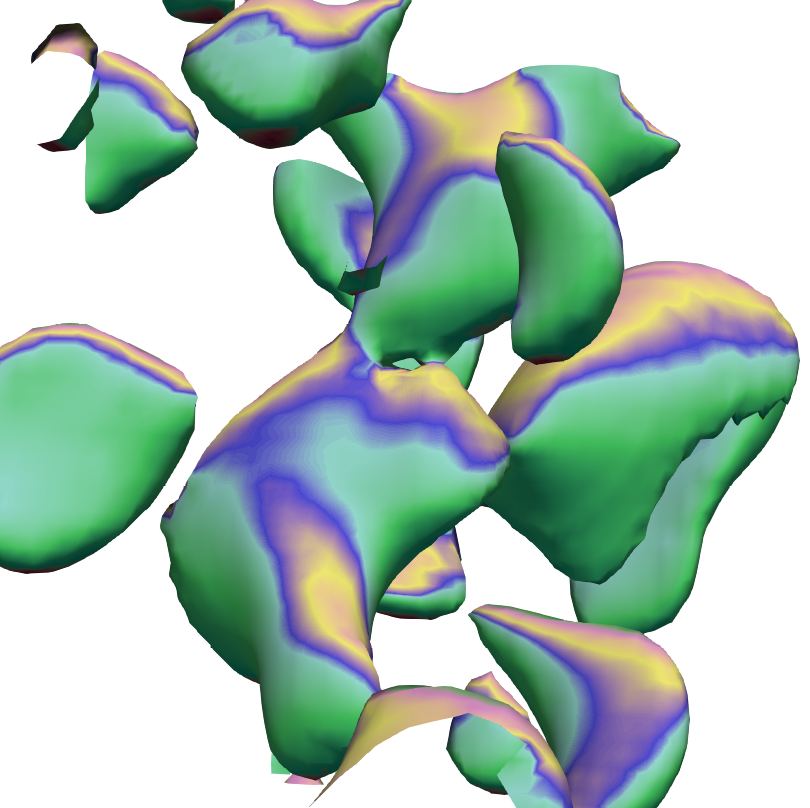
\includegraphics[width=0.16\linewidth]{isocontour/isocontour-signature}}
	\subcaptionbox{\emph{reference}}
	{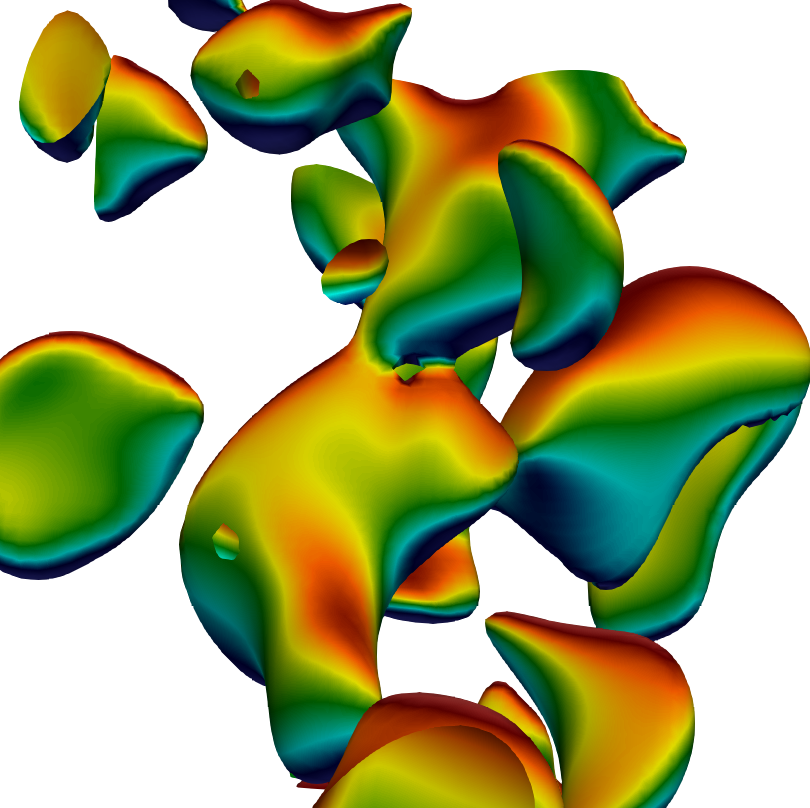
\includegraphics[width=0.16\linewidth]{isocontour/isocontour-groundtruth}} \caption{Rendering of
	isosurfaces at isovalue of 0.2, at 0.4 bps. The surfaces are colored by the x component of the
	normal vector at each point. The surfaces reconstructed by $s_{wav}$ and $s_{iso-sig}$ are closest to the reference, followed by $s_{bit}$, $s_{mag}$, and $s_{lvl}$.}
	\label{fig:isocontour-surfaces-pressure}
\end{figure*}

\begin{figure}[h]
	\centering
	\subcaptionbox{\emph{by bit plane} ($s_{bit}$)}
	{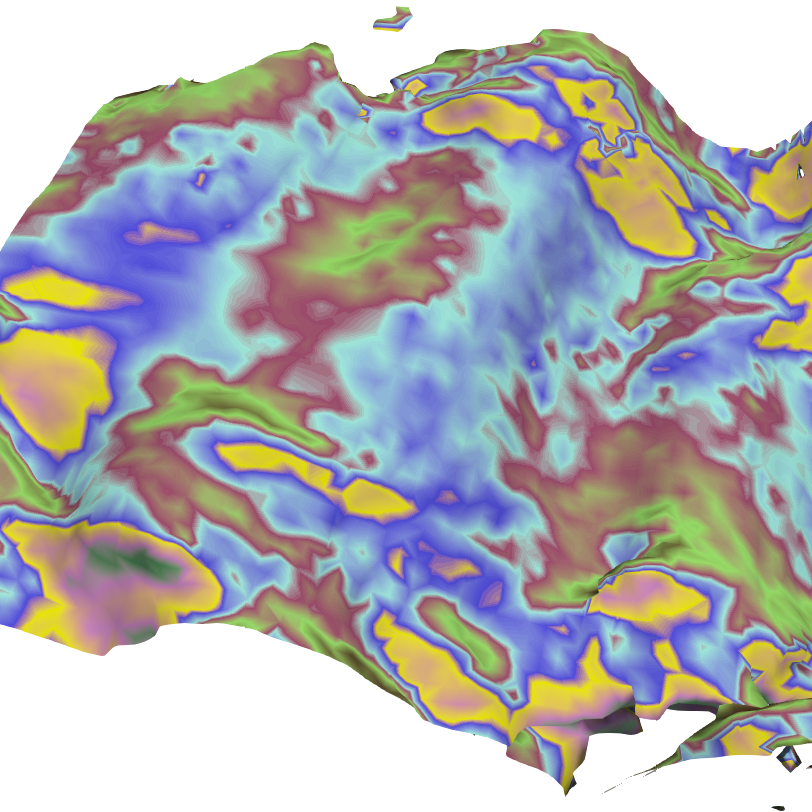
\includegraphics[width=0.31\linewidth]{isocontour/isocontour2-bit-plane}}
	\subcaptionbox{\emph{by wavelet norm} ($s_{wav}$)}
	{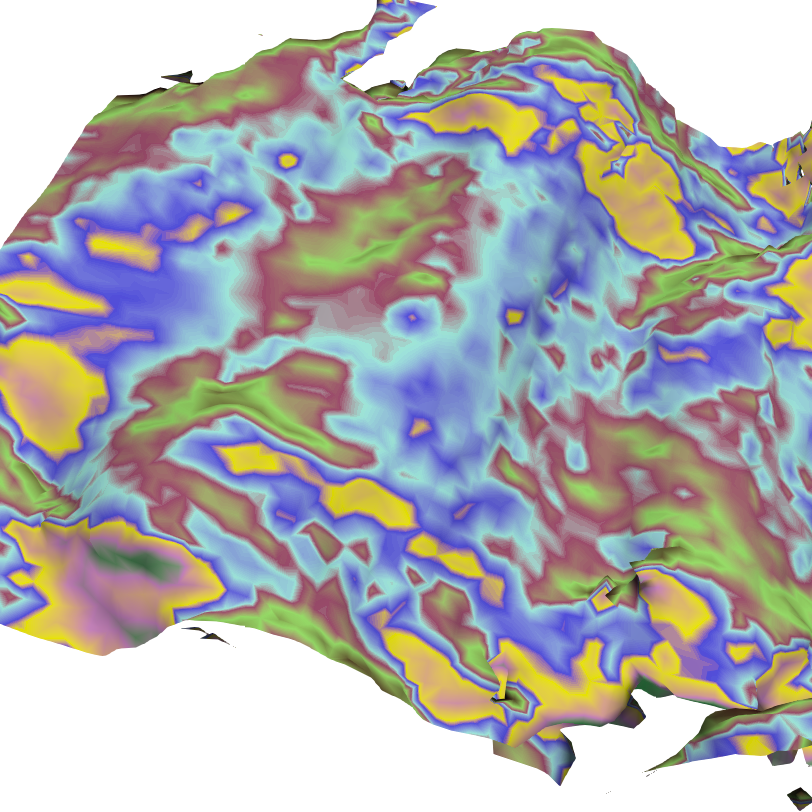
\includegraphics[width=0.31\linewidth]{isocontour/isocontour2-wavelet-norm}}
	\subcaptionbox{\emph{reference}}
	{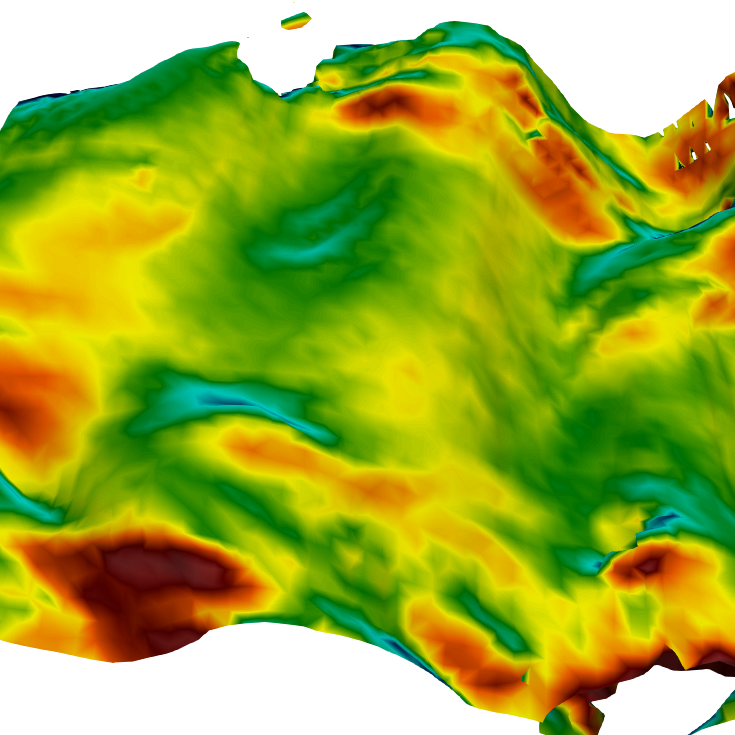
\includegraphics[width=0.31\linewidth]{isocontour/isocontour2-groundtruth}}
	\caption{\emph{Plasma}'s isosurface reconstructed at 0.3 bps.}
	\label{fig:isocontour-surfaces-plasma}
\end{figure}

Extraction of isosurfaces is an essential task in any visualization and analysis system. For
example, in a combustion simulation, isosurfaces of OH concentration can separate burning and
extinguished regions. In medical imaging, organs can also be separated from the background with
isosurface extraction. Beyond visualization, topological methods such as the Reeb graph [CITE] show the
evolution of level sets by identifying equivalence classes of isosurfaces. Among other applications,
Reeb graphs are used in topological simplification and surface segmentation.

In attempting to define an error metric to compare isosurfaces, we have found that the popular
Hausdorff distance [CITE] is not very robust --- it varies drastically with minor changes in the
surfaces. Etiene \etal propose using several geometrical~\cite{verifiable-isosurface} and
topological~\cite{topology-verification-isosurface} metrics for verification of isosurfaces. In this
paper, we have chosen a simple metric that assumes nothing about the surfaces, that is the number of
misclassified voxels in the volume. Given a volume and an isovalue, we assign the label 0 to samples
that are less than or equal to the isovalue, and label the rest 1. Samples of the reconstructed
volume are labeled the same way. The distance between the two isosurfaces is then the number of
voxels that are labeled differently between the two volumes.

The metric defined above, however, does not properly measure the importance of a packet, if the
error caused by switching off a packet is too small (in orders of subvoxel). Obtaining accurate
measurements of such errors is a crucial step in~\Cref{alg:greedy}. We, therefore, amend the
error metric based on misclassified voxels, by adding to it the relative difference in area between
the two isosurfaces. This relative difference is computed using the formula $|A_1-A_2|/A(_1)$, where
$A_1$ and $A_2$ are isosurface reas. The normalization reduces the range of this term to $[0, 1]$.
The idea is that when the number of misclassified voxels is less than $1$, the subvoxel error is
instead captured by this relative difference in surface areas.

With the error metric defined, we compute a data-dependent stream optimized for that metric
($s_{iso-opt}$) and a stream based on its signature ($s_{iso-sig}$) using~\Cref{alg:greedy}
and~\Cref{alg:signature}. \Cref{fig:isocontour-plots} compares the performances of these two
streams, along with $s_{bit}$, $s_{lvl}$, $s_{wav}$, and $s_{mag}$. Both $s_{lvl}$ and $s_{mag}$
perform poorly, indicating that isosurface extraction favors resolution over precision. There are
crossovers between $s_{bit}$ and $s_{wav}$ for the \emph{plasma} data set.

For this data set, the isosurface is extracted from a region with a low gradient, which means the
surface is very sensitive to low-ordered bits (i.e., a slight change in values moves the isosurface
by larger distance). For this reason, the $s_{wav}$ stream initially performs better, as it streams
more precision bits. As $s_{bit}$ acquires enough precision, however, it starts to resolve the
fine-scale geometry of the surface better than $s_{wav}$ does
(from~\Cref{fig:bit-plane-vs-wavelet-norm-gradient} in~\Cref{sec:gradient}, we learned that
$s_{wav}$ tends to reconstruct a smoother function everywhere).

In~\Cref{fig:isocontour-surfaces-plasma} we render the surfaces reconstructed by $s_{bit}$ and
$s_{wav}$ at 0.3 bps, which confirms that $s_{bit}$ is able to preserve better the fine-scale
featureas on the surface. For the \emph{turbulence} field, the isosurface is extracted from a
high-gradient region; thus precision bits matter less, and $s_{bit}$ outperforms $s_{wav}$ from the
beginning. $s_{bit}$ also outperforms $s_{iso-sig}$ in this case, because local signatures coming
from regions where the isosurface does not intersect will dilute those coming from regions where it
does. This phenomenon makes the signature less useful for tasks that involve localization in spatial
domain, such as isosurface extraction. Here, it happens in various degrees for every data set but it
is especially relevant in the case of \emph{turbulence}, since the surface is confined to very small
regions of the whole volume.

For a typical isosurface that is relatively smooth and is not too confined to small regions, such as
\emph{pressure} with an isovalue of 0.2, $s_{wav}$ typically outperforms $s_{bit}$
(see~\Cref{fig:isocontour-surfaces-pressure}). This figure renders the isosurfaces reconstructed at
0.4 bps for all streams. In terms of the quality of the reconstructed surfaces, $s_{iso-sig} \approx
s_{wav} > s_{bit} > s_{mag} > s_{lvl}$, which agrees with the curves in
~\Cref{fig:isocontour-plots}a. 
